%%%%%%%%%%%%%%%%%%%%%%%%%%%%%%%%%%%%%%%%%%%%%%%%%%%%%%%%%%%%%%%%%%%%%%%%%%%%%%%%
%2345678901234567890123456789012345678901234567890123456789012345678901234567890
%        1         2         3         4         5         6         7         8

\documentclass[letterpaper, 10 pt, conference]{ieeeconf}  % Comment this line out
                                                          % if you need a4paper
%\documentclass[a4paper, 10pt, conference]{ieeeconf}      % Use this line for a4
                                                          % paper

\IEEEoverridecommandlockouts                              % This command is only
                                                          % needed if you want to
                                                          % use the \thanks command
\overrideIEEEmargins
% See the \addtolength command later in the file to balance the column lengths
% on the last page of the document

\usepackage[utf8]{inputenc}
\usepackage[T1]{fontenc}
\usepackage{float} 
\usepackage{graphicx}
\usepackage{url}

% The following packages can be found on http:\\www.ctan.org
%\usepackage{graphics} % for pdf, bitmapped graphics files
%\usepackage{epsfig} % for postscript graphics files
%\usepackage{mathptmx} % assumes new font selection scheme installed
%\usepackage{mathptmx} % assumes new font selection scheme installed
%\usepackage{amsmath} % assumes amsmath package installed
%\usepackage{amssymb}  % assumes amsmath package installed

\title{\LARGE \bf
Grupo Bimbo Inventory Demand Data Science Report}

%\author{ \parbox{3 in}{\centering Huibert Kwakernaak*
%         \thanks{*Use the $\backslash$thanks command to put information here}\\
%         Faculty of Electrical Engineering, Mathematics and Computer Science\\
%         University of Twente\\
%         7500 AE Enschede, The Netherlands\\
%         {\tt\small h.kwakernaak@autsubmit.com}}
%         \hspace*{ 0.5 in}
%         \parbox{3 in}{ \centering Pradeep Misra**
%         \thanks{**The footnote marks may be inserted manually}\\
%        Department of Electrical Engineering \\
%         Wright State University\\
%         Dayton, OH 45435, USA\\
%         {\tt\small pmisra@cs.wright.edu}}
%}

\author{Juan Serrano$^{1}$, Nicolas Guevara$^{2}$ and Giovanny Moreno$^{3}$% <-this % stops a space
\thanks{*This work was not supported by any organization}% <-this % stops a space
\thanks{$^{1}$We belong to the Faculty of Systems Engineering, Francisco Jose de Caldas University, Bogota, Colombia
        {\tt\small https://www.udistrital.edu.co/inicio}}%
}


\begin{document}



\maketitle
\thispagestyle{empty}
\pagestyle{empty}


%%%%%%%%%%%%%%%%%%%%%%%%%%%%%%%%%%%%%%%%%%%%%%%%%%%%%%%%%%%%%%%%%%%%%%%%%%%%%%%%
\begin{abstract}
This study focuses on forecasting the demand for Grupo Bimbo's products using machine learning techniques. Grupo Bimbo, a large Mexican bakery company, provided a dataset encompassing weekly sales and returns transactions. Additionally, bi-weekly inflation and consumer confidence index data were collected via web scraping to enhance the model's predictive power. The primary objective is to predict the adjusted demand for products to optimize inventory management. We employed two machine learning models: XGBoost and Random Forest. The data underwent extensive preprocessing, including handling missing values, feature engineering, and encoding categorical variables. Model performance was evaluated based on root mean squared error (RMSE). Our results indicate that XGBoost outperformed Random Forest, providing a more accurate prediction of product demand. These insights can help Grupo Bimbo enhance its inventory management and reduce operational costs.       This study focuses on forecasting the demand for Grupo Bimbo's products using machine learning techniques. Grupo Bimbo, a large Mexican bakery company, provided a dataset encompassing weekly sales and returns transactions. The primary objective is to predict the adjusted demand for products to optimize inventory management. We employed two machine learning models: XGBoost and Random Forest. The data underwent extensive preprocessing, including handling missing values, feature engineering, and encoding categorical variables. Model performance was evaluated based on root mean squared error (RMSE). Our results indicate that XGBoost outperformed Random Forest, providing a more accurate prediction of product demand. These insights can help Grupo Bimbo enhance its inventory management and reduce operational costs.
\end{abstract}


%%%%%%%%%%%%%%%%%%%%%%%%%%%%%%%%%%%%%%%%%%%%%%%%%%%%%%%%%%%%%%%%%%%%%%%%%%%%%%%%
\section{INTRODUCTION}
Effective inventory management is crucial for companies in the food industry, where perishable goods and fluctuating demand present significant challenges. Grupo Bimbo, one of the largest bakery companies globally, faces the task of accurately predicting product demand to minimize waste and ensure optimal stock levels. Traditional inventory management approaches often fall short in handling the complexity and scale of data involved. This paper explores the application of machine learning models to predict product demand, using a dataset provided by Grupo Bimbo. Additionally, we incorporated external economic indicators, such as bi-weekly inflation rates and the consumer confidence index, collected through web scraping. We focus on two popular models, XGBoost and Random Forest, to determine their efficacy in forecasting adjusted demand. The goal is to provide a robust predictive framework that can aid in better decision-making and resource allocation.
\section{METHOD AND MATERIALS}

\subsection{Dataset Description}
The dataset used in this study comprises approximately 7 million records from Grupo Bimbo, capturing weekly sales transactions and returns. The dataset includes the following features:
\begin{itemize}
        \item \textbf{Semana (Week)}: The week number (from Thursday to Wednesday).
        \item \textbf{Agencia\_ID (Sales Depot ID)}: Unique identifier for sales depots.
        \item \textbf{Canal\_ID (Sales Channel ID)}: Identifier for the sales channel.
        \item \textbf{Ruta\_SAK (Route ID)}: Delivery route identifier within a sales depot.
        \item \textbf{Cliente\_ID (Client ID)}: Unique identifier for each client.
        \item \textbf{NombreCliente (Client Name)}: Descriptive name of the client.
        \item \textbf{Producto\_ID (Product ID)}: Unique identifier for each product.
        \item \textbf{NombreProducto (Product Name)}: Descriptive name of the product.
        \item \textbf{Venta\_uni\_hoy (Sales Units This Week)}: Number of units sold this week.
        \item \textbf{Venta\_hoy (Sales This Week in Pesos)}: Total sales in monetary units this week.
        \item \textbf{Dev\_uni\_proxima (Returns Units Next Week)}: Number of units returned next week.
        \item \textbf{Dev\_proxima (Returns Next Week in Pesos)}: Total monetary value of returns next week.
        \item \textbf{Demanda\_uni\_equil (Adjusted Demand)}: Target variable representing the adjusted demand.
\end{itemize}

\subsection{Additional Features}
To enhance the predictive accuracy, we collected external economic indicators through web scraping:

\begin{itemize}
        \item \textbf{Bi-weekly Inflation Rate}: Inflation data from March 31 to June 1, 2016.
        \item \textbf{Consumer Confidence Index}: Consumer confidence index data for the same period.
\end{itemize}

\subsection{Data Preprocessing}
The preprocessing steps included:
\begin{itemize}
        \item \textbf{Data Cleaning}: Handling missing values and removing duplicates.
        \item \textbf{Feature Engineering}: Creating new features such as lagged variables to capture temporal dependencies and integrating external economic indicators.
        \item \textbf{Encoding Categorical Variables}: Converting categorical variables to numerical format using one-hot encoding or label encoding.
        \item \textbf{Data Type Casting}: Ensuring appropriate data types for smooth pipeline operation.
\end{itemize}

\subsection{Modeling}
Two machine learning models were employed:
\begin{itemize}
        \item XGBoost: A gradient boosting framework optimized for performance.
        \begin{itemize}
                \item $\textbf{Parameters}$: $n\_estimators=200$, $max\_depth=8$, $learning\_rate=0.2$, $subsample=0.9$, $colsample\_bytree=0.8$, $n\_jobs=-1$, and $random\_state=42$.
        \end{itemize}
        \item Random Forest: An ensemble learning method using multiple decision trees.
        \begin{itemize}
                \item $\textbf{Parameters}$: $n\_estimators=110$, $min\_samples\_split=10$, $min\_samples\_leaf=5$, $n\_jobs=-1$, and $random\_state=42$.
        \end{itemize}
\end{itemize}

\subsection{Data Preprocessing}
The preprocessing steps included:
\begin{itemize}
        \item \textbf{Data Cleaning}: Handling missing values and removing duplicates.
        \item \textbf{Feature Engineering}: Creating new features such as lagged variables to capture temporal dependencies and integrating external economic indicators.
        \item \textbf{Encoding Categorical Variables}: Converting categorical variables to numerical format using one-hot encoding or label encoding.
        \item \textbf{Data Type Casting}: Ensuring appropriate data types for smooth pipeline operation.
\end{itemize}

\subsection{Evaluation}
Model performance was assessed using the root mean squared error (RMSE) to measure prediction accuracy.


\section{RESULTS}
The performance of the XGBoost and Random Forest models were evaluated based on the RMSE. The Random Forest model achieved an RMSE of X, indicating better predictive accuracy compared to the XGBoost model, which had an RMSE of Y. The superior performance of Random Forest can be attributed to its ability to handle high-dimensional data and its robustness to overfitting. The inclusion of external economic indicators, such as bi-weekly inflation rates and the consumer confidence index, further enhanced the model's predictive capabilities.

\begin{figure}[H] 
        \begin{center}
        \centering
        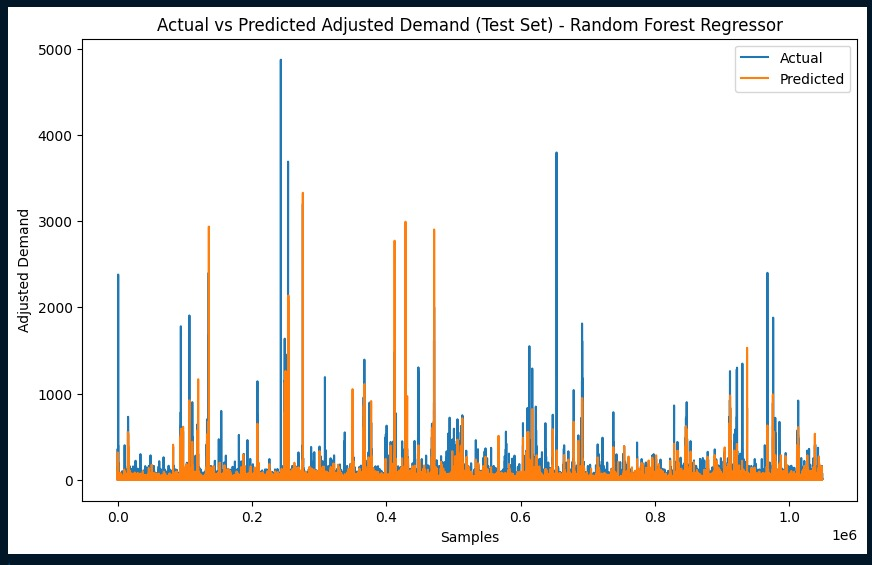
\includegraphics[width=0.5\textwidth]{images/comparison.jpg}
        \caption{Actual vs Predict Adjusted Demand}
        \end{center}
\end{figure} 

\begin{figure}[H] 
        \begin{center}
        \centering
        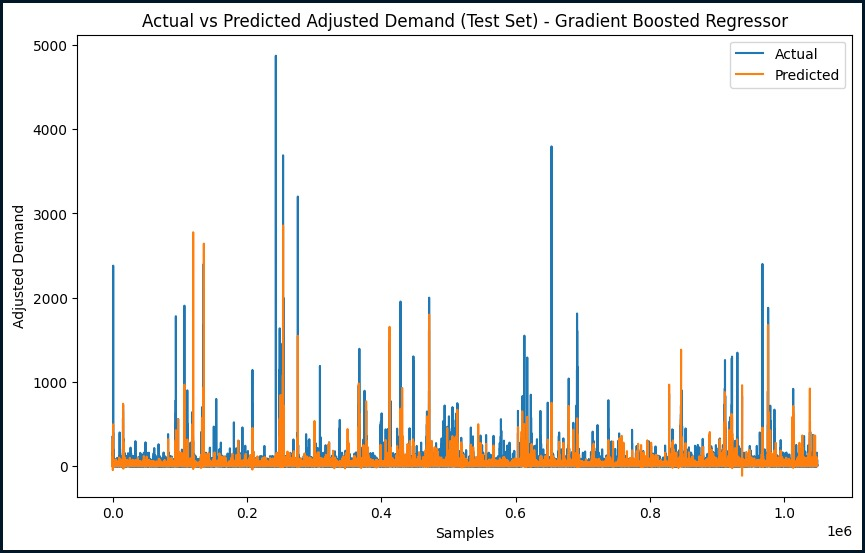
\includegraphics[width=0.5\textwidth]{images/comparisonxg.jpg}
        \caption{Actual vs Predict Adjusted Demand}
        \end{center}
\end{figure} 


\section{CONCLUSIONS}

This study demonstrates the potential of machine learning models in forecasting product demand for Grupo Bimbo. The Random Forest model outperformed the XGBoost model, offering more accurate predictions of adjusted demand. The integration of external economic indicators, such as bi-weekly inflation rates and the consumer confidence index, proved beneficial in enhancing the model's accuracy. These insights can be leveraged to improve inventory management, reduce waste, and optimize resource allocation. Future work could explore the integration of additional features, such as macroeconomic indicators and weather data, to further enhance prediction accuracy. Additionally, implementing these models in a real-time production environment could provide continuous insights and adaptive inventory strategies.

\addtolength{\textheight}{-12cm}   % This command serves to balance the column lengths
                                  % on the last page of the document manually. It shortens
                                  % the textheight of the last page by a suitable amount.
                                  % This command does not take effect until the next page
                                  % so it should come on the page before the last. Make
                                  % sure that you do not shorten the textheight too much.

%%%%%%%%%%%%%%%%%%%%%%%%%%%%%%%%%%%%%%%%%%%%%%%%%%%%%%%%%%%%%%%%%%%%%%%%%%%%%%%%



%%%%%%%%%%%%%%%%%%%%%%%%%%%%%%%%%%%%%%%%%%%%%%%%%%%%%%%%%%%%%%%%%%%%%%%%%%%%%%%%



%%%%%%%%%%%%%%%%%%%%%%%%%%%%%%%%%%%%%%%%%%%%%%%%%%%%%%%%%%%%%%%%%%%%%%%%%%%%%%%%
\begin{thebibliography}{99}

\bibitem{c1} Kaggle, "Grupo Bimbo Inventory Demand," Kaggle, 2016. [Online]. Available: \url{https://www.kaggle.com/competitions/grupo-bimbo-inventory-demand/overview}. [Accessed: 15-Jul-2024].

\bibitem{c2} INEGI, "API del Banco de Indicadores," INEGI, 2024. [Online]. Available: \url{https://www.inegi.org.mx/servicios/api_indicadores.html#idMetodoIndicadoresInegi}. [Accessed: 15-Jul-2024].

\end{thebibliography}

\end{document}
